\section{The Regulator's Design Problem}
\label{sec:regulator}

The preceding sections characterize a firm's response to a given audit design. We now ask what threshold a regulator should choose, anticipating that response, treating $p_H$, $\rho$, $\delta$, $f$, $L$ as exogenous features of the audited population. Suppose the regulator's objective is long-run quality, $W(\tau)$, defined by Theorem~\ref{prop:recurring}'s three cases:
\begin{equation}
W(\tau) =
\begin{cases}
q^*(p_L) & \tau \leq q^*(p_L) \quad \text{[Case (a)]} \\
\bar{q}_B(\tau) & q^*(p_L) < \tau < q^*(p_H) \quad \text{[Case (b)]} \\
q^*(p_H) & \tau \geq q^*(p_H) \quad \text{[Case (c)]}
\end{cases}
\label{eq:regulatorobjective}
\end{equation}
where $\bar{q}_B(\tau)$ is $\bar{q}_B(\tau,\rho)$ from Corollary~\ref{cor:aggwelfare} with $\rho=0.30$ fixed throughout this section.

\begin{proposition}[Boundary regions are flat]
$W(\tau) = q^*(p_L)$ for every $\tau \leq q^*(p_L)$, and $W(\tau) = q^*(p_H)$ for every $\tau \geq q^*(p_H)$. (Immediate from Theorem~\ref{prop:recurring}: in Case (a), long-run quality is $q^*(p_L)$ regardless of the specific $\tau$; in Case (c), it is $q^*(p_H)$ regardless of the specific $\tau$, since the firm converges there without ever reaching $\tau$, including at $\tau=q^*(p_H)$ itself.)
\label{prop:flatregions}
\end{proposition}

So the design question lives entirely in Case (b), where we lack a general proof that $\bar{q}_B(\tau)$ is monotonic. Sweeping $\tau$ across $(0.30,1.55)$ at $\rho=0.30$ (Figure~\ref{fig:tausweep}), $\bar{q}_B(\tau)$ increases at every sampled point, from $W=0.427$ at $\tau=0.40$ to $W=1.487$ at $\tau=1.50$, just below $q^*(p_H)=1.542$, with no reversal. Combined with Proposition~\ref{prop:flatregions}, welfare is non-decreasing across the entire range, attaining its maximum $q^*(p_H)$ at $\tau^\star=q^*(p_H)$ and beyond — a numerically-supported trend, not a proven limit.

This maximum is degenerate: at $\tau\geq q^*(p_H)$ certification is never granted (Case (c)), so ``$\tau^\star=q^*(p_H)$'' is indistinguishable from eliminating the safe harbor outright, not a design recommendation — and not because the firm invests nothing there, since it still invests $c_\delta>0$ forever (Appendix~\ref{app:extra-sim} checks this against a cost-adjusted objective and finds the recommendation robust). The substantive content is that welfare rises monotonically through the achievable Case (b) range, approaching but never exceeding $q^*(p_H)$: a regulator wanting the safe harbor to remain operative should target $\tau$ close to, but strictly below, $q^*(p_H)$. Since $q^*(p_H)$ depends only on cost structure and drift, not $\rho$, it can be estimated from firm behavior under negligible safe-harbor effects (e.g., early in an enforcement regime) — a concrete target distinct from calibrating $\tau$ to a population-wide norm, closer to how the four-fifths rule was historically set.

\begin{figure}[t]
\centering
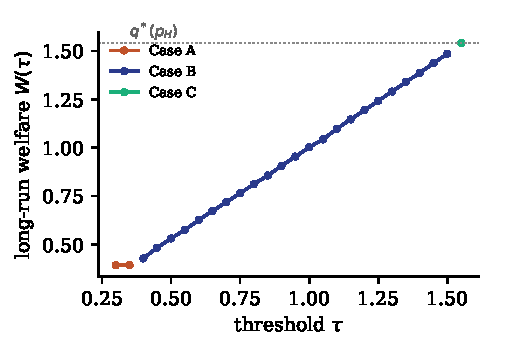
\includegraphics[width=0.55\linewidth]{figures/fig_tausweep.pdf}
\caption{Long-run welfare $W(\tau)$ as the threshold varies, $\rho=0.30$ fixed. Flat below $q^*(p_L)$ and at or above $q^*(p_H)$ (Proposition~\ref{prop:flatregions}, proven); numerically monotonic in between (Case B), approaching $q^*(p_H)$ at the upper boundary.}
\label{fig:tausweep}
\end{figure}
